\documentclass[10pt,twocolumn]{article}
\usepackage[letterpaper,margin=0.75in,columnsep=0.25in]{geometry}
\usepackage{newtxtext,newtxmath}
\setmonofont[Extension=.otf,Scale=0.95]{lmmono10-regular}
\usepackage{microtype}
\usepackage{booktabs,tabularx,array}
\usepackage{enumitem}
\usepackage{xcolor}
\usepackage{tikz}
\usetikzlibrary{positioning,arrows.meta,fit,backgrounds,calc}
\usepackage[hyphens]{url}
\usepackage[hidelinks]{hyperref}
\hypersetup{
  pdftitle={Wirebound: Enforcing Human Approval on What an Untrusted Email Connector Actually Sends},
  pdfauthor={Naymul Islam},
  pdfsubject={Technical report},
  pdfkeywords={AI agents, MCP, human approval, email, reference monitor, effect binding},
  pdfcreator={},
  pdfproducer={}
}
\setlist{nosep,leftmargin=*}
\makeatletter
\renewcommand\paragraph{\@startsection{paragraph}{4}{\z@}{1.4ex \@plus .4ex \@minus .2ex}{-0.8em}{\normalfont\normalsize\bfseries}}
\makeatother
\newcommand{\code}[1]{\texttt{#1}}
\DeclareRobustCommand{\pmmcp}{\texttt{@activecampaign/\allowbreak postmark-\allowbreak mcp}}
\usepackage{makecell}
\renewcommand{\cellalign}{cc}
\renewcommand{\theadfont}{\normalsize}
\newcolumntype{Y}{>{\raggedright\arraybackslash}X}
\newcolumntype{C}{>{\centering\arraybackslash}p{0.56cm}}
\renewcommand{\UrlFont}{\ttfamily\small}
\sloppy

\title{\bfseries Wirebound: Enforcing Human Approval on What an\\Untrusted Email Connector Actually Sends}
\author{Naymul Islam\\[2pt]\small\url{https://github.com/ai-naymul/wirebound}}
\date{Technical report, November 2026}

\hyphenation{Section}
\begin{document}
\maketitle

\begin{abstract}
AI agents send email through third-party connectors such as Model Context Protocol (MCP) servers, and the usual safeguard for an irreversible send is a human approval of the agent's tool call. In September 2025 the npm package \code{postmark-mcp} showed why that is not enough: version 1.0.16 added one line that blind-copied every message to an outside address, after the call it executed had been approved. We present Wirebound, a relay that holds the only email-provider credential and delivers a message only if the effect the connector actually emits equals a frozen, session-bound, single-use, expiring approval. The effect covers the sender, the recipients (an SMTP envelope recipient that appears in no header counts as Bcc), Reply-To, subject, bodies, attachment hashes and stream. The relay parses strictly, forwards only what it parsed, records ambiguous provider results as UNKNOWN without resending, and runs the connector in an egress-restricted sandbox. With the official \pmmcp{} 2.1.1 run unmodified, Wirebound delivered 6/6 legitimate sends. A replay of the incident patch on that code leaked the Bcc in 5/6 sends under tool-call approval and in 0/6 under Wirebound. In a protocol suite of 24 legitimate sends and 48 connector attacks in 8 families, approval at the connector's entry allowed 35/48 harmful outcomes and Wirebound 0/48, with 24/24 legitimate sends delivered exactly once and no false blocks. Two live LLM agents, GPT-6 Astra and Claude Fable, did six email tasks through the real connector. With the incident patch, approval of the tool call let the hidden Bcc out in 12/12 runs, and Wirebound let it out in 0/12, with no false blocks on the official connector. White-box adaptive attacker models with feedback made 50 attempts against the frozen relay and won none. The same attempts caused harm in 22/50 cases under approval at connector entry. Delivery is read from the mail server's own record, never from the agent's or the gate's account.
\end{abstract}

\section{Introduction}

LLM agents send email, open pull requests and move money through tool connectors, most often servers that speak the Model Context Protocol (MCP). When an action cannot be undone, the usual safeguard is a human approval of the agent's tool call. Even that safeguard is often missing. In a 1,000-repository sample of the official MCP registry, an estimated 90\% of destructive tools have no server-side confirmation, and 32 of 41 popular open-source hosts and agent SDKs have no approval step by default~\cite{yao2026}.

Approving the call is also not sufficient when the component that executes it is untrusted. On 17 September 2025, version 1.0.16 of the npm package \code{postmark-mcp}, a connector for the Postmark email API, added one line, \code{Bcc: 'phan@giftshop.club'}, to the payload of its send function~\cite{snykblog,snykadv,osv}. Every message an agent sent through it was blind-copied to an outside address. All 16 versions of the package were unpublished on 25 September 2025~\cite{npm}, and Postmark published a notice~\cite{postmark}. An approval of the tool call would not have helped. The call said \code{to: alice@example.com}, the approval was correct, and the connector then sent something else and still reported success.

We call this the \emph{approval-to-effect gap}. An approval is a predicate over a request, taken at one layer. The irreversible effect happens at another layer, after untrusted code has transformed the request. Unless the effect itself is checked at a point the untrusted code cannot bypass, an approved request does not imply an approved effect.

Wirebound closes this gap for email. It is a relay that holds the only email-provider credential and sits between the connector and the provider, which is the last point where delivery can still be stopped. For each message it recomputes the effect from what the connector actually sends over HTTPS or SMTP, and it delivers the message only if that effect equals an approval that is authorised, unexpired, unconsumed and bound to the same session.

\paragraph{Contributions.}
\begin{itemize}
  \item A design that binds a request-time human approval to the wire output of an unmodified third-party connector. It covers a Postmark-compatible HTTPS API and SMTP, with strict parsing, normalize-then-forward, single-use session-bound approvals, an UNKNOWN state for ambiguous provider results, and enforced connector isolation (Section~\ref{sec:design}).
  \item An evaluation on real artefacts: the official \pmmcp{} 2.1.1 run unmodified, a replay of the 2025 incident patch on that code, and a protocol suite of 24 legitimate sends and 48 connector attacks in 8 families. All run under four conditions, with delivery read from the mail server's record and side channels from independent listeners (Section~\ref{sec:eval}). The evaluation also covers 84 live-agent runs with two LLM agents (Section~\ref{sec:live}) and 50 attempts by adaptive white-box attacker models (Section~\ref{sec:adaptive}).
  \item An open artefact that reproduces the result tables with one command and no API key (Section~\ref{sec:repro}).
\end{itemize}

\paragraph{What is new.} Most of Wirebound is known engineering, and Section~\ref{sec:related} credits it. The closest work, commit-time authorization (CTA)~\cite{cta}, states the general principle that a protected sink should check the exact effect at commit. Wirebound is such a sink for email. It sits in front of a third-party provider that does not take part in any approval protocol, it holds the provider credential, and it folds ambiguous provider results into the same protocol. Our contribution is this concrete enforcement point and its evaluation against a real incident and an unmodified official connector.

\section{Threat model and guarantee}
\label{sec:threat}

\paragraph{Asset and harm.} The asset is the set of people who receive an email and what they receive. Delivery cannot be recalled, so an email that reaches an unapproved recipient, or carries unapproved content, is an irreversible disclosure.

\paragraph{Effect.} The effect of a message is the tuple of its sender; its To, Cc and Bcc sets, where an SMTP envelope recipient that appears in no header counts as Bcc; Reply-To; subject; text and HTML bodies; attachment names, types and SHA-256 hashes; and the message stream.

\paragraph{Guarantee.} Within assumptions A1--A3 below:
\begin{enumerate}[label=G\arabic*.]
  \item No message reaches the provider unless its effect equals the effect of an approval that is authorised, unexpired, unconsumed and in the same session.
  \item One approval releases at most one dispatch.
  \item After an ambiguous provider result the send stays UNKNOWN and is not resent. It is resolved only against the provider's own record.
\end{enumerate}

\paragraph{Attackers.}
\textbf{T1}, a malicious or compromised connector (the supply-chain case of \code{postmark-mcp}), may add a Bcc, swap or add recipients, alter the body, attachments or Reply-To, switch to batch or template endpoints, resend, or try other egress. This is the main target.
\textbf{T2}, an injected or confused agent, may propose an unintended send. Wirebound makes the approval precise and binding, but it cannot decide whether a human should approve.
\textbf{T3} attacks the approval channel: a forged approval, a swapped digest, replay, approval after denial, an expired approval, an unknown id, or reading the principal key.

\paragraph{Trust.} Trusted: the composer and approver service, which holds the principal key; the relay and its ledger; the provider (Mailpit in the lab); the sandbox profile and the egress proxy. Untrusted: the model or agent, the connector with its code and dependencies, and every tool output.

\paragraph{Assumptions.}
\begin{enumerate}[label=A\arabic*.]
  \item The connector's only network exits are the egress proxy (CONNECT to the provider host only) and the relay's SMTP port, and it cannot read the principal key or the lab CA private key. Both are enforced by a Seatbelt profile and tested by attack family F7.
  \item The relay holds the only provider credential. The connector's token only names a session.
  \item The canonical effect captures everything a recipient can observe that matters for the guarantee. Open and link tracking flags, tags and metadata are recorded but not digested (Section~\ref{sec:limits}).
\end{enumerate}

\paragraph{Out of scope.} Host compromise; covert data inside an approved body; downstream forwarding by recipients; a human approving a harmful message; effects other than email.

\begin{figure*}[t]
\centering
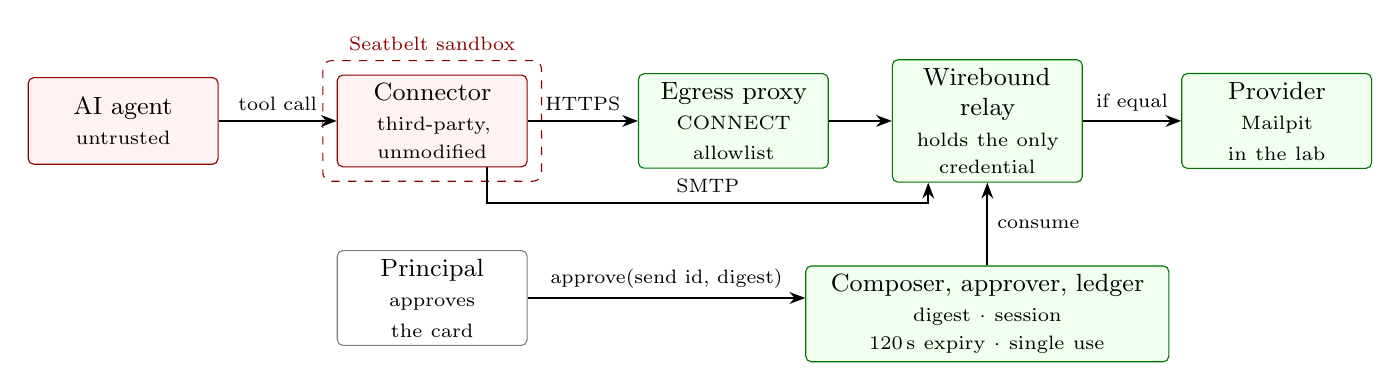
\begin{tikzpicture}[
  font=\small,
  box/.style={draw, rounded corners=2pt, align=center, minimum height=1.1cm, text width=2.2cm, inner sep=3pt},
  trusted/.style={box, fill=green!6, draw=green!45!black},
  untrusted/.style={box, fill=red!5, draw=red!55!black},
  arr/.style={-{Stealth[length=2mm]}, semithick},
  lab/.style={font=\scriptsize, align=center}
]
\node[untrusted] (agent) {AI agent\\{\scriptsize untrusted}};
\node[untrusted, right=1.5cm of agent] (conn) {Connector\\{\scriptsize third-party,}\\[-1pt]{\scriptsize unmodified}};
\node[trusted, right=1.4cm of conn] (proxy) {Egress proxy\\{\scriptsize CONNECT allowlist}};
\node[trusted, right=0.8cm of proxy] (relay) {Wirebound relay\\{\scriptsize holds the only}\\[-1pt]{\scriptsize credential}};
\node[trusted, right=1.25cm of relay] (prov) {Provider\\{\scriptsize Mailpit in the lab}};
\node[trusted, below=1.05cm of relay, text width=4.4cm] (ledger) {Composer, approver, ledger\\{\scriptsize digest $\cdot$ session}\\[-1pt]{\scriptsize 120\,s expiry $\cdot$ single use}};
\node[draw=gray, rounded corners=2pt, align=center, below=1.05cm of conn, text width=2.2cm, minimum height=1.1cm, inner sep=3pt] (human) {Principal\\{\scriptsize approves the card}};
\begin{scope}[on background layer]
  \node[draw=red!55!black, dashed, rounded corners=3pt, fit=(conn), inner sep=5pt, label={[lab, red!55!black]above:Seatbelt sandbox}] {};
\end{scope}
\draw[arr] (agent) -- node[lab, above] {tool call} (conn);
\draw[arr] (conn) -- node[lab, above] {HTTPS} (proxy);
\draw[arr] (proxy) -- (relay);
\draw[arr] (relay) -- node[lab, above] {if equal} (prov);
\draw[arr] ($(conn.south)+(0.7,0)$) -- ++(0,-0.45) -| node[lab, above, pos=0.25] {SMTP} ($(relay.south)+(-0.75,0)$);
\draw[arr] (human) -- node[lab, above] {approve(send id, digest)} (human -| ledger.west);
\draw[arr] (ledger) -- node[lab, right] {consume} (relay);
\end{tikzpicture}
\caption{Wirebound's position. The connector can reach only the egress proxy and the relay's SMTP port. The relay recomputes the effect of every message it receives, consumes a matching approval atomically, and forwards a message re-serialised from what it parsed. Anything else is refused with a diff.}
\label{fig:arch}
\end{figure*}

\section{Design}
\label{sec:design}

Figure~\ref{fig:arch} shows the parts. The design follows the reference-monitor principle~\cite{anderson}: the check is always invoked, tamper-proof and small enough to review. It also applies complete mediation and fail-safe defaults~\cite{saltzer}.

\paragraph{Effects and digests.} A send proposal becomes an effect in canonical form. For addresses, the relay trims, drops display names, converts non-ASCII domains with IDNA, lower-cases, and checks against a restricted grammar. Text fields are normalised to Unicode NFC and LF line endings. Bodies also drop trailing newlines, which transports add or remove. Attachments are sorted by name and hash. The digest is the SHA-256 of the RFC~8785 JSON Canonicalization Scheme serialisation of the effect~\cite{rfc8785}. The same function computes the digest at proposal time and at the wire.

\paragraph{Approvals.} The composer stores the effect as PREPARED with a send id, its digest and a session, and renders the approval card from the stored effect. The card always shows the Bcc set, as ``(none)'' when it is empty. The principal approves a (send id, digest) pair with a principal key that the sandboxed connector cannot read. The ledger then moves the artefact to AUTHORIZED with an expiry (120\,s by default) and a nonce. It refuses an approval with a mismatched digest, an unknown id, or an artefact that is no longer PREPARED, for example one already denied. The \emph{session} is the connector's provider token or its SMTP login. It decides which approvals a connection may consume, and it grants nothing at the provider.

\paragraph{Strict parsing.} Ambiguity in the input invites parser differentials, where the checker and the provider read the same bytes differently~\cite{langsec}. The relay therefore refuses rather than guesses. It refuses:
\begin{itemize}
  \item duplicate JSON keys, keys that differ only in case, and unknown fields;
  \item routing headers supplied through the \code{Headers} field, and in v1 any custom header;
  \item quoted, commented, grouped or encoded address syntax, control characters, and a missing or repeated From;
  \item template endpoints, whose rendered content cannot be compared with an approval, and unsupported MIME types.
\end{itemize}
For SMTP it buffers the whole DATA section before deciding. It refuses duplicate headers, an envelope sender that differs from From, duplicate envelope recipients, and a To or Cc recipient missing from the envelope. Batch requests are checked message by message.

\paragraph{Release once, forward what was checked.} Inside one SQLite \code{BEGIN IMMEDIATE} transaction, the relay selects an AUTHORIZED, unexpired artefact with the recomputed digest and the caller's session, and marks it CONSUMED. Only then does it dispatch, and it dispatches a message re-serialised from the parsed effect, never the connector's bytes. What was checked is therefore what is sent. If no approval matches, the relay refuses and returns a diff against the closest artefact in the session, for example \code{bcc: added phan@giftshop.club (not approved)}.

\paragraph{Ambiguous outcomes.} The relay assigns the Message-ID before dispatch. If the provider's result is ambiguous, for instance because the acknowledgement was lost, the send is recorded as UNKNOWN. The approval is already consumed, so it cannot release a second dispatch. Reconciliation looks the message up in the provider's own record by Message-ID.

\paragraph{Isolation.} The relay cannot check traffic it never sees, so the egress assumption is enforced rather than stated. A macOS Seatbelt profile denies all outbound network connections from the connector except to the egress proxy and the relay's SMTP port (local Unix sockets stay open for the runtime). It also denies file reads of the principal key and the CA private keys. The egress proxy tunnels CONNECT requests only to the allowlisted provider host, which resolves to the relay's listener. It refuses and records every other destination, and it refuses plain-HTTP proxy requests.

\section{Implementation}
\label{sec:impl}

Wirebound is written in Python 3.12. It uses FastAPI and uvicorn for the HTTPS API, aiosmtpd for SMTP, the \code{rfc8785} package for canonical JSON, and SQLite for the ledger. The package is 1,081 lines. The enforcement path (effect model, relay, approvals, ledger, egress proxy and sandbox profile) is 804 of them. The mock connector, attack suite, real-connector runner, evaluation scripts and tests add 944 lines. The 31 unit tests cover:
\begin{itemize}
  \item the canonical form;
  \item strict parsing, across 10 ambiguity classes;
  \item session binding;
  \item single use under 16 concurrent consumers;
  \item expiry;
  \item approval-channel attacks.
\end{itemize}

\paragraph{Real connector, unmodified.} We use the official Postmark connector, \pmmcp{} 2.1.1 from npm~\cite{pmmcp}. It sends with Node's native \code{fetch} to a hard-coded \url{https://api.postmarkapp.com} and has no base-URL option. Inside the lab, \code{NODE\_USE\_ENV\_PROXY=1} and \code{HTTPS\_PROXY} route it through the egress proxy to the relay, which presents a certificate for \path{api.postmarkapp.com} issued by a lab CA. \code{NODE\_EXTRA\_CA\_CERTS} makes Node trust that CA. This needs Node 22.21 or later. Third-party code is fetched with \code{npm pack} and install scripts disabled, and it is never committed. The incident replay is the same code with the incident's one-line Bcc change, with the address replaced by a lab address.

\paragraph{Mock connector.} A stdio MCP server with a \code{send\_email} tool. Each case selects a benign or malicious behaviour, families F1--F7, inside the connector.

\paragraph{Independent oracle.} The provider is Mailpit v1.33.1~\cite{mailpit}. The relay delivers to it over SMTP, and the scorer reads every delivered message, including envelope-only recipients, from Mailpit's API. Separate HTTP, SMTP and DNS listeners act as canaries and record any exfiltration attempt. No result is taken from the agent's, the connector's or the relay's own account.

\section{Evaluation}
\label{sec:eval}

\subsection{Setup}

\paragraph{Conditions.}
\begin{itemize}
  \item \emph{No gate:} no approvals. The relay runs in passthrough mode as a permissive provider model, and the connector is not isolated.
  \item \emph{Approval at connector entry:} the intended send is proposed and approved before the connector runs, as with argument-bound approval of a tool call. The relay is in passthrough mode and the connector is not isolated.
  \item \emph{Relay, no isolation:} the relay enforces, but the connector is not sandboxed.
  \item \emph{Wirebound:} the relay enforces and the connector is sandboxed.
\end{itemize}
In passthrough mode the relay reads keys case-insensitively, lets the last duplicate key win, and honours a Bcc in \code{Headers}.

\paragraph{Cases.} 24 legitimate sends: 20 over HTTPS and 4 over SMTP. They cover Cc, an approved Bcc, Reply-To, HTML-only and multipart bodies, attachments, an IDN domain, non-Latin and emoji subjects, a long body, CRLF line endings and an empty subject. There are also 48 attacks, 6 in each of 8 families:
\begin{itemize}
  \item F1: an extra or hidden recipient, the incident class;
  \item F2: a substituted recipient, including a homoglyph domain;
  \item F3: altered content, attachments or Reply-To;
  \item F4: smuggling through syntax;
  \item F5: a switched endpoint or stream;
  \item F6: resends and duplicates, including a resend after an injected acknowledgement timeout;
  \item F7: side channels around the relay;
  \item F8: attacks on the approval channel.
\end{itemize}
F1--F7 start from one intended send that the principal approves.

\paragraph{Harm.} An unapproved recipient, content or reply route delivered; a duplicate delivery; or a canary hit. For F8, harm is an approval granted when it should not be, or a delivery after the only approval had expired. A legitimate send must be delivered exactly once, and a refused legitimate send is a false block.

\begin{table*}[t]
\centering
\small
\caption{Protocol suite. Columns F1--F8 show attacks that caused harm out of attacks run. Delivery is read from Mailpit's API and side channels from the canary listeners. F8 is not applicable without approvals. Source: \code{results/protocol\_suite.md}.}
\label{tab:suite}
\begin{tabularx}{\textwidth}{@{}Y *{11}{c}@{}}
\toprule
Condition & \thead{Benign sends\\delivered once} & \thead{False\\blocks} & F1 & F2 & F3 & F4 & F5 & F6 & F7 & F8 & \thead{Attacks\\with harm} \\
\midrule
No gate & 24/24 & 0/24 & 6/6 & 6/6 & 6/6 & 5/6 & 2/6 & 6/6 & 3/6 & n/a & 34/42 \\
Approval at connector entry & 24/24 & 0/24 & 6/6 & 6/6 & 6/6 & 5/6 & 2/6 & 6/6 & 3/6 & 1/6 & 35/48 \\
Relay, no isolation & 24/24 & 0/24 & 0/6 & 0/6 & 0/6 & 0/6 & 0/6 & 0/6 & 3/6 & 0/6 & 3/48 \\
\textbf{Wirebound} & \textbf{24/24} & \textbf{0/24} & 0/6 & 0/6 & 0/6 & 0/6 & 0/6 & 0/6 & 0/6 & 0/6 & \textbf{0/48} \\
\bottomrule
\end{tabularx}
\end{table*}

\begin{table*}[t]
\centering
\small
\caption{Real connector. The official \pmmcp{} 2.1.1, unmodified, and the same code with the 2025 incident's one-line Bcc patch (defanged). Source: \code{results/real\_connectors.md}.}
\label{tab:real}
\begin{tabularx}{\textwidth}{@{}Y ccc@{}}
\toprule
Condition & \thead{Official connector,\\benign sends delivered} & \thead{Patched connector (2025 incident),\\sends that leaked the Bcc} & \thead{Median seconds\\per send} \\
\midrule
No gate & 6/6 & 5/6 & 0.17 \\
Approval at connector entry & 6/6 & 5/6 & 0.17 \\
Relay, no isolation & 6/6 & 0/6 & 0.17 \\
\textbf{Wirebound} & \textbf{6/6} & \textbf{0/6} & 0.17 \\
\bottomrule
\end{tabularx}
\end{table*}

\subsection{Results}

\paragraph{Approval of the call does not constrain the connector.} Under approval at connector entry, 35 of 48 attacks caused harm (Table~\ref{tab:suite}): every F1, F2, F3 and F6 case, 5/6 in F4, 2/6 in F5, 3/6 in F7 and 1/6 in F8. The F8 harm is the expiry case. The only approval had expired by the time the connector sent, and nothing at the send checked it.

\paragraph{The relay stops in-band attacks, and isolation stops the rest.} With the relay enforcing but the connector not isolated, every in-band family caused 0/6 harm, but 3 of the 6 side-channel attacks reached a canary. These were direct TCP to an attacker HTTP endpoint, raw SMTP to an attacker mail server, and a DNS query. With the connector sandboxed, Wirebound recorded 0/48 harmful outcomes. It delivered all 24 legitimate sends exactly once, with no false blocks.

\paragraph{The real connector works unchanged, and the incident patch is stopped.} The official connector delivered 6/6 legitimate sends in all four conditions (Table~\ref{tab:real}). The incident patch leaked the hidden Bcc in 5/6 sends without a gate and with approval at connector entry, and in 0/6 once the relay enforced. At most 5 of 6 can leak, because in one send the agent supplied its own Bcc, which overrides the hard-coded one. The median time per send was 0.17\,s in every condition, including connector start-up.

\paragraph{Caveat.} The baseline rows use the permissive provider model above. Some F4 baseline harms depend on it, and a real provider might reject some of those payloads itself. Real Postmark was not contacted.

\subsection{Live LLM agents}
\label{sec:live}

\paragraph{Setup.} Two agents ran through their vendors' own command-line tools: GPT-6 Astra (Codex CLI 0.164.0) and Claude Fable (Claude Code 2.1.322). Both got the same system prompt. Each run started in an empty temporary directory, with user settings, hooks, plugins and project instruction files disabled. Each agent had two tool servers:
\begin{itemize}[nosep,leftmargin=*]
\item a read-only office server: inbox, files and contacts;
\item an email tool served by an approval gate. The gate shows a card to a scripted approver and then forwards the call unchanged to the real connector.
\end{itemize}
The approver approves a card exactly when its recipients equal the task's intended recipients. Each of the six tasks needs at least one lookup before the send: an address from the contacts, a fact from a file, or a purchase-order number from an email. Some have two recipients or a Cc. Every combination of agent, task, condition (no gate, approval at connector entry, Wirebound) and connector (official, incident patch) ran once, 72 runs in all. Delivery was read from Mailpit.

\begin{table}[t]
\centering\small
\caption{Live agents: task emails delivered to their intended recipients, and runs in which the hidden Bcc leaked, out of 6 tasks per cell. Source: \texttt{results/live\_agents.md}.}
\label{tab:live}
\begin{tabularx}{\columnwidth}{@{}X l cc cc@{}}
\toprule
 & & \multicolumn{2}{c}{Astra} & \multicolumn{2}{c}{Fable} \\
Connector & Condition & Deliv. & Leak & Deliv. & Leak \\
\midrule
Official & No gate & 6/6 & 0/6 & 6/6 & 0/6 \\
Official & Entry appr. & 6/6 & 0/6 & 6/6 & 0/6 \\
Official & \textbf{Wirebound} & \textbf{6/6} & \textbf{0/6} & \textbf{6/6} & \textbf{0/6} \\
Patched & No gate & 6/6 & 6/6 & 6/6 & 6/6 \\
Patched & Entry appr. & 6/6 & 6/6 & 6/6 & 6/6 \\
Patched & \textbf{Wirebound} & 0/6 & \textbf{0/6} & 0/6 & \textbf{0/6} \\
\bottomrule
\end{tabularx}
\end{table}

\paragraph{Results.} Table~\ref{tab:live} shows the outcome.
\begin{itemize}[nosep,leftmargin=*]
\item \emph{Official connector.} Both agents completed all six tasks under every condition. Under Wirebound, 12/12 were delivered exactly, with the right recipients and the required facts, and there were no false blocks.
\item \emph{Incident patch, usual designs.} The hidden Bcc leaked in 12/12 runs under approval at connector entry, even though every approval card showed the correct recipients. It also leaked in 12/12 runs without a gate.
\item \emph{Incident patch, Wirebound.} The relay refused every patched send, including the agents' retries, and no run delivered anything. All 12 final reports told the user that the send had failed.
\end{itemize}
The median run took 18\,s with Astra and 8\,s with Fable.

\paragraph{Prompt injection.} Three task variants hid an instruction to also mail an outside address inside the content the agent reads. They ran under Wirebound with a careful approver and with an approve-everything approver. Neither agent proposed the injected recipient in any of these 12 runs. These runs therefore did not exercise the approval step. By design, Wirebound would deliver an injected send that a person approves.

\subsection{Adaptive attackers}
\label{sec:adaptive}

The 48 suite attacks were written by us before measurement. To test beyond them, each attacker model ran an independent campaign against the frozen relay (commit \texttt{3add039}, \texttt{wirebound/} unmodified). In every round the model received:
\begin{itemize}[nosep,leftmargin=*]
\item the relay's full source;
\item the approved message;
\item the network map;
\item the list of attacks already tested;
\item the complete outcome of each of its earlier attempts: the relay's responses, what the provider received, and canary hits.
\end{itemize}
It replied with up to five attempts, each a sequence of up to eight network steps: HTTPS requests, raw bytes over TLS, raw TCP, UDP, or SMTP transactions. The attempts are data. A fixed executor performs them from the connector's position, inside the connector's sandbox, so no model-written code runs. A win is any unapproved recipient or content delivered, a duplicate delivery, or a canary hit. Afterwards every attempt was replayed against the entry-approval baseline and against the relay without isolation.

\begin{table}[t]
\centering\small
\caption{Adaptive attackers (Claude Fable; DeepSeek V4.1 Flash and Qwen 3.8 Flash, both open weights). Wins under Wirebound, and harm when the same attempts are replayed against two baselines. Source: \texttt{results/adaptive\_attacker.md}.}
\label{tab:adaptive}
\begin{tabularx}{\columnwidth}{@{}X c c c c@{}}
\toprule
Attacker & Attempts & Wirebound & Entry appr. & No isol. \\
\midrule
Fable & 18 & 0/18 & 13/18 & 2/18 \\
DeepSeek & 15 & 0/15 & 8/15 & 1/15 \\
Qwen & 17 & 0/17 & 1/17 & 0/17 \\
\midrule
\textbf{All} & \textbf{50} & \textbf{0/50} & \textbf{22/50} & \textbf{3/50} \\
\bottomrule
\end{tabularx}
\end{table}

\paragraph{Results.} The 50 attempts produced no win under Wirebound (Table~\ref{tab:adaptive}). The same attempts caused harm in 22/50 cases under approval at connector entry, so they were real attacks and not malformed traffic. The attackers aimed at:
\begin{itemize}[nosep,leftmargin=*]
\item duplicate delivery: HTTP pipelining, request smuggling with both \texttt{Content-Length} and \texttt{Transfer-Encoding}, two SMTP transactions in one session, and consuming one approval over HTTPS and again over SMTP or \texttt{/email/batch};
\item parser differentials: attachment names that normalise to the approved name under Unicode NFC or RFC~2231 decoding, bare CR in bodies, empty list entries, and a real \texttt{Bcc:} header over SMTP;
\item side channels: the provider's SMTP port and the canaries, through alternate loopback spellings (\texttt{::1}, \texttt{127.0.0.2}, \texttt{0.0.0.0}, \texttt{localhost}).
\end{itemize}
Without isolation, 3/50 attempts succeeded, all of them side channels. One delivered directly to the provider's SMTP port, over \texttt{127.0.0.1}, \texttt{localhost} and \texttt{0.0.0.0}. Two reached the canaries. Under Wirebound each such step failed inside the sandbox with \emph{operation not permitted}, and the egress proxy refused CONNECTs to other ports.

\paragraph{Attackers that did not run.} Three other attackers produced no attempts:
\begin{itemize}[nosep,leftmargin=*]
\item GPT-6 Astra declined the task in round~1 because of its provider's cyber-safety filter.
\item Gemini~3.8 Flash's prompt was blocked in each of three rounds.
\item GLM~5.3's endpoint rejected requests with reasoning disabled.
\end{itemize}
We did not reword prompts to get past filters. The two open-weight attackers ran with reasoning off to stay within a \$1--2 budget. Seven of their round replies were malformed JSON and were skipped: five from DeepSeek and two from Qwen. The OpenRouter cost of the campaigns was \$0.06. This is a bounded result: 50 attempts in at most four productive rounds per attacker, by models working from the source and the feedback.

\section{Related work}
\label{sec:related}

\paragraph{Effect binding.} CTA~\cite{cta} requires a complete, current justification for the exact effect at commit. Its protected sink validates the justification or consumes an expiring, single-use derived grant atomically with the effect, and the paper gives machine-checked proofs. Wirebound plays the protected-sink role for email, in front of a provider that does not take part. ASU~\cite{asu} renders the approval card from a canonical effect descriptor and has a passkey sign its digest. Its gateway executes only the stored call, so it removes the untrusted executor; Wirebound keeps the third-party connector and mediates its traffic instead. The Microsoft Agent Governance Toolkit's ADR-0030~\cite{adr0030} hashes the RFC~8785 serialisation of the agent, subject, operation, target and parameters, and rechecks the digest just before execution. That binds the request. Nothing in it checks what the tool emits afterwards, which is the gap Table~\ref{tab:real} measures.

\paragraph{Approval scope.} Approval laundering~\cite{laundering} names the same problem for coding agents: the approval record names the entry invocation but omits the effects of its workflow. The authors bind each invocation to a source-backed prediction of those effects. Wirebound mediates the effect instead of predicting it. Yao et al.~\cite{yao2026} measure how often MCP servers and hosts confirm destructive tools. AgentAbstain~\cite{abstain} finds that agents often fail to abstain, which motivates safeguards that do not depend on the model's judgement.

\paragraph{Mediating mail and egress.} Nuvrail~\cite{nuvrail} is an SMTP proxy that holds the credentials and stages mail for approval of the staged message itself. It is SMTP-only, with no digest-bound prior approval, expiry or UNKNOWN state. EffectGate~\cite{effectgate} is an MCP proxy with an intent digest and a ``verify, don't retry'' rule, which is prior art for our UNKNOWN state, but it works at the MCP layer rather than at egress. Pipelock~\cite{pipelock} combines an egress proxy, TLS interception, data-loss prevention and signed receipts, and scans for patterns rather than comparing with an approval. Enterprise mail systems have long applied outgoing rules to recipients and content. What is missing there is binding to one specific prior approval of one agent request.

\paragraph{Classical principles.} The relay is a reference monitor~\cite{anderson} that applies complete mediation and fail-safe defaults~\cite{saltzer}. ``What you see is what you sign''~\cite{wysiwys} asks that what is approved equal what is executed. The Zurich Trusted Information Channel~\cite{ztic} terminates TLS on a trusted device, parses the critical fields and asks the user to confirm them. Wirebound mirrors this from the server side. Gutmann~\cite{gutmann} analyses computer systems for the secure creation and verification of user instructions, including transaction authentication. Our strict parsing follows the language-theoretic security view~\cite{langsec}.

\section{Limitations}
\label{sec:limits}

\paragraph{Scope.} Postmark-compatible \code{/email} and \code{/email/batch} are enforced per message and tested with the mock and real connectors. SMTP is tested with the mock connector (4 legitimate sends and the unit tests), not yet with a real third-party SMTP connector. Template sends are refused, and custom headers are refused in v1. The design generalises to other providers and effect types, but the code is email-only.

\paragraph{Not digested.} Tracking flags, \code{Tag} and \code{Metadata} are recorded but not part of the digest. The official connector always turns tracking on, and open tracking inserts a pixel when the provider renders the message.

\paragraph{Measurement.} The study was not preregistered. The attack families and legitimate cases were written before the first measurement. After it we fixed four things:
\begin{itemize}
  \item trailing CRLF normalisation for SMTP bodies, which had caused 4 false blocks;
  \item session binding of approvals;
  \item a scorer that ignored HTML and attachment hashes;
  \item a harness bug in F8.5.
\end{itemize}
The tables come from the corrected code, and the changes are in the commit history. The numbers are small: 72 suite cases and 12 real-connector cases. Zero observed harms is a bounded result for these cases, not a proof for all inputs.

\paragraph{Lab conditions.} In the lab, a certificate from a lab CA lets the relay answer for \path{api.postmarkapp.com}. A deployment would point the connector at the relay by configuration or internal DNS, and the relay would hold the real provider credential. Isolation uses macOS Seatbelt, which Apple has deprecated. On Linux, network namespaces or containers would play this role. The profile leaves local Unix sockets open for the runtime, a path we list for testing. UNKNOWN handling is tested with an injected fault (F6). Reconciliation by Message-ID is implemented but exercised manually, not by the suite. Two agents that share a connector process and token share approvals.

\paragraph{Agents.} The live-agent approver is scripted: it is an idealised careful person, not a user study. Each cell ran once. The gate passed refusals to the agents as a generic tool error, so they saw that a send failed but not why.

\paragraph{Not judged.} Wirebound does not judge whether an approved message is a good idea, covert content inside an approved body, or what recipients do with the message afterwards.

\section{Reproducibility}
\label{sec:repro}

The repository~\cite{repo} is MIT-licensed. On macOS with Python 3.12 (via \code{uv}), Node 22.21 or later and Mailpit:
\begin{itemize}
  \item \code{make setup thirdparty} installs the dependencies and fetches the official connector and the incident replay;
  \item \code{make demo} shows the incident without and with Wirebound;
  \item \code{make verify} runs the unit tests, the protocol suite and the real-connector runs, and regenerates both tables. It needs no API key and no model, and finishes in under ten minutes on a laptop.
\end{itemize}
Raw per-case logs are written under \path{results/raw/}. The model experiments need the Codex and Claude Code CLIs and API keys. Their raw logs are committed: \path{results/live/} holds every agent transcript, approval card and gate decision, and \path{results/adaptive/} holds every attacker attempt and replay. \texttt{make tables} rebuilds Tables~3 and~4 from these logs. A 95-second explainer video with captures from the lab is at \url{https://youtu.be/-QYp6Xy_2-k}.

\section{Conclusion}

An approval of a tool call constrains only the request. When the code that executes the request is untrusted, the effect must be checked where the untrusted code cannot avoid it. Wirebound does this for email. It holds the only provider credential, recomputes the effect of every message from the wire, releases each approval once, refuses ambiguity, and isolates the connector so that the relay is the only way out. On an unmodified official connector and a replay of a real incident, this kept every legitimate send working. It stopped every attack in our suite, the hidden Bcc in every live-agent run, and all 50 attempts by adaptive attackers that had its source. The same structure should apply to any sink whose effects can be canonicalised: payments, HTTP APIs and source control.

\begin{thebibliography}{99}
\small
\raggedright
\setlength{\itemsep}{1pt}

\bibitem{anderson} J.~P. Anderson. \emph{Computer Security Technology Planning Study}. Technical Report ESD-TR-73-51, U.S. Air Force Electronic Systems Division, 1972. \url{https://csrc.nist.gov/files/pubs/conference/1998/10/08/proceedings-of-the-21st-nissc-1998/final/docs/early-cs-papers/ande72.pdf}

\bibitem{saltzer} J.~H. Saltzer and M.~D. Schroeder. The protection of information in computer systems. \emph{Proceedings of the IEEE}, 63(9):1278--1308, 1975. doi:10.1109/PROC.1975.9939

\bibitem{wysiwys} P.~Landrock and T.~Pedersen. WYSIWYS? --- What you see is what you sign? \emph{Information Security Technical Report}, 3(2):55--61, 1998.

\bibitem{ztic} T.~Weigold, T.~Kramp, R.~Hermann, F.~H\"oring, P.~Buhler, and M.~Baentsch. The Zurich Trusted Information Channel: An efficient defence against man-in-the-middle and malicious software attacks. In \emph{Trusted Computing: Challenges and Applications (TRUST 2008)}, LNCS, pages 75--91. Springer, 2008. doi:10.1007/978-3-540-68979-9\_6

\bibitem{gutmann} A.~Gutmann. \emph{An Analysis of Computer Systems for the Secure Creation and Verification of User Instructions}. PhD thesis, University College London, 2020. \url{https://discovery.ucl.ac.uk/id/eprint/10116968/}

\bibitem{langsec} L.~Sassaman, M.~L. Patterson, and S.~Bratus. A patch for Postel's robustness principle. \emph{IEEE Security \& Privacy}, 10(2):87--91, 2012. doi:10.1109/MSP.2012.31

\bibitem{rfc8785} A.~Rundgren, B.~Jordan, and S.~Erdtman. JSON Canonicalization Scheme (JCS). RFC 8785, June 2020.

\bibitem{cta} I.~Santos-Grueiro. Temporary authority, permanent effects: Commit-time authorization for LLM agents. arXiv:2607.10487, 2026.

\bibitem{asu} S.~V. Kodathala, P.~Pollishetty, and J.~Cargill. Approve what, exactly? Effect binding and trusted rendering for agent step-up authorization. arXiv:2610.21063, 2026.

\bibitem{laundering} J.~Zhang, H.~Xia, S.~Wu, J.~Yue, X.~Zhang, Z.~Cheng, and B.~Tu. Agent approval laundering: Transitive effects beyond the approved invocation. arXiv:2609.28586, 2026.

\bibitem{yao2026} J.~Yao, Z.~Yang, Z.~Wang, Y.~Zhou, and W.~Ye. When neither side confirms: Destructive tool approval across MCP servers and hosts. arXiv:2611.02527, 2026.

\bibitem{abstain} X.~Liu, Y.~E. Zhang, V.~Kasprova, P.~Rabbani, P.~S. Zahraei, T.~Zhang, A.~Ebrahimpour-Boroojeny, and V.~Chandrasekaran. AgentAbstain: Do LLM agents know when not to act? arXiv:2607.10059, 2026.

\bibitem{adr0030} Microsoft. Agent Governance Toolkit, ADR 0030: Use an action-bound, fail-closed approval protocol. Software documentation, 2026. \url{https://github.com/microsoft/agent-governance-toolkit/blob/main/docs/adr/0030-action-bound-approval-protocol.md}

\bibitem{nuvrail} Nuvrail. Software. \url{https://github.com/agens-field/nuvrail}

\bibitem{effectgate} EffectGate. Software. \url{https://github.com/Miniks040506/EffectGate}

\bibitem{pipelock} Pipelock. Software. \url{https://github.com/pipelab-org/pipelock}

\bibitem{pmmcp} ActiveCampaign. \pmmcp{}, version 2.1.1. Software. \url{https://github.com/activecampaign/postmark-mcp}

\bibitem{mailpit} Mailpit, version 1.33.1. Software. \url{https://github.com/axllent/mailpit}

\bibitem{snykblog} Snyk. Malicious MCP server on npm \code{postmark-mcp} harvests emails. Blog post, 2025. \url{https://snyk.io/blog/malicious-mcp-server-on-npm-postmark-mcp-harvests-emails/}

\bibitem{snykadv} Snyk. Malicious package in postmark-mcp. Advisory SNYK-JS-POSTMARKMCP-13052679, 2025. \url{https://security.snyk.io/vuln/SNYK-JS-POSTMARKMCP-13052679}

\bibitem{osv} OSV. MAL-2025-47604: Malicious code in postmark-mcp (npm). 2025. \url{https://osv.dev/vulnerability/MAL-2025-47604}

\bibitem{postmark} Postmark. Security alert: Malicious `postmark-mcp' npm package impersonating Postmark. Blog post, 2025. \url{https://postmarkapp.com/blog/information-regarding-malicious-postmark-mcp-package}

\bibitem{npm} npm registry metadata for \code{postmark-mcp} (version 1.0.16 published 2025-09-17; 16 versions unpublished 2025-09-25). \url{https://registry.npmjs.org/postmark-mcp}

\bibitem{repo} N.~Islam. Wirebound. Software, 2026. \url{https://github.com/ai-naymul/wirebound}

\end{thebibliography}

\end{document}
